\chapter{羧酸的衍生物}

\section{物理性质}


\subsection{酰卤}

\begin{center}
    \chemfig{R-[:30]C(=[:90]O)-[:-30]X}
\end{center}

不能形成分子间的氢键。

\subsection{酯、酸酐}

\begin{center}
    \chemfig{R-[:30]C(=[:90]O)-[:-30]OR}
\end{center}

\begin{center}
    \chemfig{R-[:30]C(=[:90]O)-[:-30]O-[:30]C(=[:90]O)-[:-30]R}
\end{center}

也不能形成氢键,低级酯一般为液体,高级酯一般为固体。
\section{化学性质}

\subsection{通性}


\begin{enumerate}
    \item 羧酸有酸性(有相对来说比较弱的亲核性)
    \item 亲核取代反应(生成羧酸衍生物)
    \item 羧酸是比较高的氧化态,可以被还原
    \item 受到羰基的影响,碳氢键也可能发生一些$\alpha - \ce{H}$异裂的反应。
    \item 脱羧反应
\end{enumerate}


\subsection{酸性}

羧酸的酸性是一种弱酸,比碳酸强。羧酸与无机酸的酸性比较:

\[
    \ce{HCl} > \ce{CH3COOH} > \ce{H2CO3}  
\]

吸电子诱导效应会导致羧酸的酸性增强。供电子诱导效应会导致羧酸的酸性减弱。

\[
    \ce{Ph-COOH} > \ce{CH3COOH}  
\]

供电子效应\scriptsize \chemfig{*6(-=-=-=)}\normalsize 比\chemfig{-[,0.5]CH_3}强


\subsection{亲核取代反应}

\subsubsection{合成酰卤$\ce{SOCl2}$、$\ce{PCl3}$}


\begin{center}
    \scriptsize
    \schemestart
    \chemfig{RCOOH} \+ $\ce{SOCl2}$ \arrow  \chemfig{R-C(=[:90]O)-Cl}
    \schemestop
\end{center}

\subsubsection{合成酸酐}

一般使用$\ce{P2O5}$。酸酐分为``外酸酐''和``内酸酐'',内酸酐主要是分子内脱水形成的酸酐。``外酸酐''可以自己和自己脱水形成酸酐,甚至可以两种不同的羧酸脱水形成``混酸酐''。

\begin{center}
    \scriptsize
    \schemestart
    \chemfig{RCOOH} \+ $\ce{SOCl2}$ \arrow  \chemfig{R-C(=[:90]O)-Cl}
    \schemestop
\end{center}


内酸酐

\begin{center}
    \scriptsize
    \schemestart
    \chemfig{*6(-=(-COOH)-(-COOH)=-=)} \+ \arrow{->[$\Delta$][$\ce{P2O5}$]}[,1.3] \chemfig{*6(-=(-C(=[:-90]O)-[:60]O?)-(-C?(=[:90]O))=-=)}
    \schemestop
\end{center}


要合成混酸酐,需要使用酰卤和酸盐来合成。

\begin{center}
    \scriptsize
    \schemestart
    \chemfig{R-[:30]C(=[:90]O)-[:-30]ONa} \+ \chemfig{Cl-[:30]C(=[:90]O)-[:-30]\textbf{R} } \arrow  \chemfig{R-[:30]C(=[:90]O)-[:-30]O-[:30]C(=[:90]O)-[:-30]\textbf{R}}
    \schemestop
\end{center}


\subsubsection{合成酯}

高中学过的反应,与醇脱水形成酯。羧酸和醇在酸催化下加热失水生成的化合物称为酯(ester)。酯化反应是可逆反应。酸脱羟基、醇脱氢比较常见,也有一些反应相反,取决于反应的历程。

\begin{center}
    \scriptsize
    \schemestart
    \chemfig{RCOOH} + $\ce{ROH}$ \arrow{->} \chemfig{R-C(=[:90]O)-OR}
    \schemestop
\end{center}


\begin{center}
    \scriptsize
    \schemestart
    \chemfig{R-C(=[:90]O)-OH} \arrow{<=>[$\ce{H+}$]} \chemfig{R-C(=[:90]O\charge{75=+}{H})-OH} \arrow{->[$\ce{ROH}$]}
    \schemestop
\end{center}

但也有少数酯化反应中,酸或醇的羟基质子化,水离去,生成酰基正离子或碳正离子中间体,该中间体再与醇或酸反应生成酯。这些反应不遵循``酸出羟基醇出氢''的规则。

\begin{figure}[H]
    \centering
    
\includegraphics[width=0.7\textwidth]{img/Fischer_esterification_mechanism.png}
\end{figure}

\subsubsection{酰胺}

\begin{center}
    \scriptsize
    \schemestart
    \chemfig{RCOOH} + $\ce{NH3}$ \arrow{->} \chemfig{R-C(=[:90]O)-NH_2}
    \schemestop
\end{center}

\subsection{还原反应}

被氢化铝锂还原为醇。

\subsection{脱羧反应}

条件:$\alpha$-C上有强吸电子基团


\subsection{$\alpha$-H取代反应}


HVZ 反应,红磷催化下,脂肪酸$\alpha$碳原子上的氢可以被卤素取代而生成$\alpha$卤代酸。

\begin{center}
    \scriptsize
    \schemestart
    \chemfig{R-CH_2-COOH} + $\ce{Br2}$ \arrow{->[P]} \chemfig{R-CH(-[:90]Br)-COOH} \arrow{->[\ch{H2O}]} \chemfig{R-CH(-[:90]OH)-COOH}
    \schemestop
\end{center}

\begin{reaction*}
    P + Br2 -> PBr3
\end{reaction*}



\section{卤代酸}

\subsection{$\alpha$-卤代酸}

卤原子受到羰基的影响,反应活性增强,因此易与各种亲核试剂发生反应,生成$\alpha$-取代羧酸。


\subsubsection{酸性}

\begin{center}
    $\ce{RCH2COOH}$ < \small\chemfig{R-CH(-[:90]Cl)-COOH} > \chemfig{R-CH(-[:90]OH)-COOH}
\end{center}


中间的羟基吸电子能力没有 $\ce{-OH}$ 强。这是因为 $\ce{-OH}$ 的氧原子还连着一个 $\ce{H}$ ,削弱了 $\ce{O}$  吸电子的能力。


\subsubsection{亲核取代}

\begin{center}
    \small
    \schemestart
    \chemfig{CH_2=CH_2} \arrow \chemfig{CH_2(-[:30]COOC_2H_5)-[:-30]COOC_2H_5}
    \schemestop
\end{center}

\subsection{$\beta$ - 卤代酸}


性质上和$\alpha$卤代酸的性质差不多。外加可以进行消去反应。


\section{羟基酸}

羟基酸的特别点一般在于其发生酯化反应时的特性。

\subsection{交酯}

两分子α-羟基酸相互发生分子间酯化形成的六元环状二酯。其中一分子羟基酸的羟基 $\ce{-OH}$ 与另一分子羟基酸的羧基 $\ce{-COOH}$ 缩合脱去一分子水生成酯,同时这一分子羟基酸的羧基 $\ce{-COOH}$ 又与另一分子羟基酸的羟基 \ce{-OH} 缩合生成另一个酯基。

\begin{figure}[h]
    \centering
    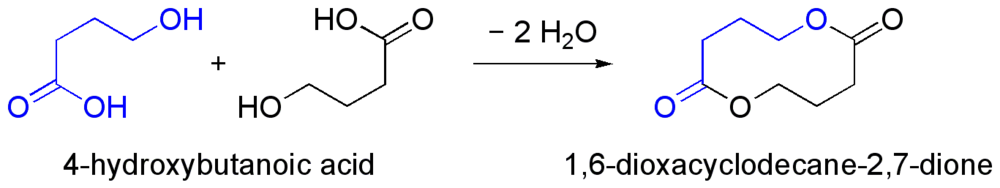
\includegraphics[width=0.8\textwidth]{img/1000px-hydroxybutanoic.png}
\end{figure}

\subsection{缩聚}

高中学的那个缩聚反应。